\clearpage
\VerdierPhysicalPageAnchor{0090}%
\VerdierSemanticAnchor{ch1-3-2-7-representing-functor-continuation}
即由 (3.1.3) 和 (3.1.7) 得到一个从 $X[1]$ 到 $W$ 的态射。这样，我们以
关于 $W$ 函子性的方式，把从 $c(p(f))$ 到 $W$ 的每个态射配到从 $X[1]$
到 $W$ 的一个态射，从而定义了态射
\VerdierSemanticAnchor{ch1-3-2-7-h-defined}
$H\colon X[1]\longrightarrow c(p(f))$。

为证明命题 (3.2.6) 的 a) 部分，只需证明：

\VerdierSemanticAnchor{ch1-3-2-7-eq2}
\begin{equation}
  \textit{态射 }JH\colon X[1]\longrightarrow X[1]
  \textit{ 是恒等态射。}
  \tag{3.2.7.2}
\end{equation}

\VerdierSemanticAnchor{ch1-3-2-7-eq3}
\begin{equation}
  \textit{态射 }HJ\colon c(p(f))\longrightarrow c(p(f))
  \textit{ 同伦于恒等态射。}
  \tag{3.2.7.3}
\end{equation}

为证明命题 (3.2.6) 的 b) 部分，还只需证明：

\VerdierSemanticAnchor{ch1-3-2-7-eq4}
\begin{equation}
  \begin{gathered}
    \textit{下图：}\\[0.35em]
    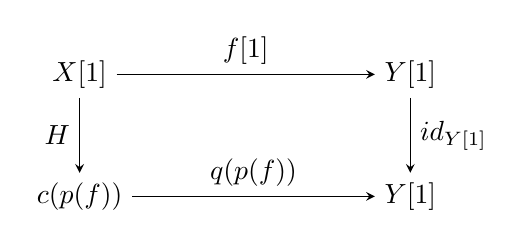
\begin{tikzpicture}[>=stealth,baseline=(current bounding box.center)]
      \node (Xs)  at (0,1.55) {$X[1]$};
      \node (Ys1) at (4.2,1.55) {$Y[1]$};
      \node (Cpf) at (0,0) {$c(p(f))$};
      \node (Ys2) at (4.2,0) {$Y[1]$};
      \draw[->] (Xs) -- node[above] {$f[1]$} (Ys1);
      \draw[->] (Xs) -- node[left] {$H$} (Cpf);
      \draw[->] (Ys1) -- node[right] {$\operatorname{id}_{Y[1]}$} (Ys2);
      \draw[->] (Cpf) -- node[above] {$q(p(f))$} (Ys2);
    \end{tikzpicture}\\[-0.15em]
    \textit{反交换。}
  \end{gathered}
  \tag{3.2.7.4}
\end{equation}

\VerdierSemanticAnchor{ch1-3-2-8}
\noindent\textbf{3.2.8. 断言 (3.2.7.2) 的证明。}\quad
\VerdierSemanticAnchor{ch1-3-2-8-jh-identity-proof}
证明态射 $JH\colon X[1]\longrightarrow X[1]$ 是恒等态射。为此，只需说明
态射 $JH$ 在由 $X[1]$ 表示的函子上诱导恒等自同态。
\VerdierSemanticAnchor{ch1-3-2-8-represented-hom-functor}
由 (3.1.3) 和 (3.1.7)，函子
\begin{equation*}
  W\longmapsto
  \operatorname{Hom}_{\operatorname{comp}(C)}(X[1],W)
\end{equation*}
就是函子：

\VerdierSemanticAnchor{ch1-3-2-8-eq1}
\begin{equation}
  W\longmapsto
  \left\{\,
  \vcenter{\hbox{%
    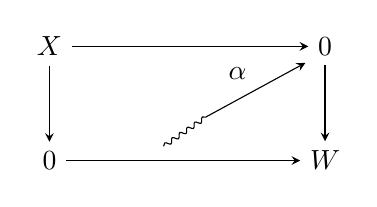
\begin{tikzpicture}[>=stealth,baseline=(current bounding box.center)]
      \node (X)  at (0,1.45) {$X$};
      \node (Z1) at (3.5,1.45) {$0$};
      \node (Z2) at (0,0) {$0$};
      \node (W)  at (3.5,0) {$W$};
      \draw[->] (X) -- (Z1);
      \draw[->] (X) -- (Z2);
      \draw[->] (Z1) -- (W);
      \draw[->] (Z2) -- (W);
      \draw[decorate,decoration={snake,amplitude=0.8pt,segment length=3.3pt}]
        (1.45,0.18) -- (2.00,0.56);
      \draw[->] (2.00,0.56) -- node[above left] {$\alpha$} (3.25,1.24);
    \end{tikzpicture}%
  }}\,\right\}.
  \tag{3.2.8.1}
\end{equation}

\VerdierSemanticAnchor{ch1-3-2-8-cpf-represented-functor}
另一方面，由 (3.2.7)，$\operatorname{comp}(C)$ 的对象 $c(p(f))$ 表示函子：

\VerdierSemanticAnchor{ch1-3-2-8-eq2}
\begin{equation}
  W\longmapsto
  \left\{\,
  \bigl(m\colon Y\longrightarrow W,\quad
  a\colon0\rightsquigarrow m,\quad
  b\colon0\rightsquigarrow mf\bigr)
  \,\right\}.
  \tag{3.2.8.2}
\end{equation}
